\documentclass{article}
\usepackage[utf8]{inputenc}
\usepackage{amsmath}
\usepackage[ruled,vlined]{algorithm2e}
\usepackage{graphicx}
\graphicspath{ {./images/} }

\title{A Semi-supervised Method for Training Deep Neural Networks}
\author{Misha Klopukh, Michael Teti, Elan Barenholtz, William Hahn}
\date{April 2019}

\begin{document}

\maketitle




\section{Abstract}

Neural networks, specifically deep convolutional networks, and supervised training by gradient descent have become the standard for artificial intelligence image recognition tasks. However, the training methods are inefficient as they change the first layers with every loss. We propose a new algorithm to pretrain neural networks that addresses these inefficiencies. XCubed is a new, gradient descent-free algorithm that can be used to pretrain CNNs layer-wise. We show that neural networks pretrained with XCubed and with some or all of the pretrained layers frozen train faster and better than networks without this training and that their training is comparable to pretrained networks.

\section{Main}

Deep Convolutional Networks trained by gradient descent have become the standard for computer vision. This approach has become popular because of the high accuracy and relatively fast training with gradient descent.\cite{alexnet}\cite{Lecun98gradient} However, there are a several fundamental flaws in how we train these networks. An image classification task can be thought of as two tasks, detection -- where image features are identified -- and classification -- where a class is decided based on detected features. These tasks in theory are separate -- you shouldn't need to change your definition of an edge or corner to learn what a cat is.\cite{something} However, in modern deep learning, we allow the network to learn its primitive features while it is learning the task. This is done because we ourselves do not know what primitive features we need to best classify objects. Features learned by gradient descent have long been shown to outperform hand-designed features.\cite{learnvcraft} However, learning these features slows down training significantly, as loss back-propagates through to the first layers and changes them often, even though the layers may have accurate features. This also causes the networks to learn more biases in the training data, and to require more data in order to learn more weights. Other problems with back-propagating through the entire network that arise more in larger networks include the vanishing gradient problem, which causes gradients at the beginning of the network to all be near zero and makes them unable to train properly.\cite{vanishinggradients}\cite{learningproblems} We propose a new way of training a neural network that mitigates these and other problems.
\newline
\begin{figure}
    \centering
    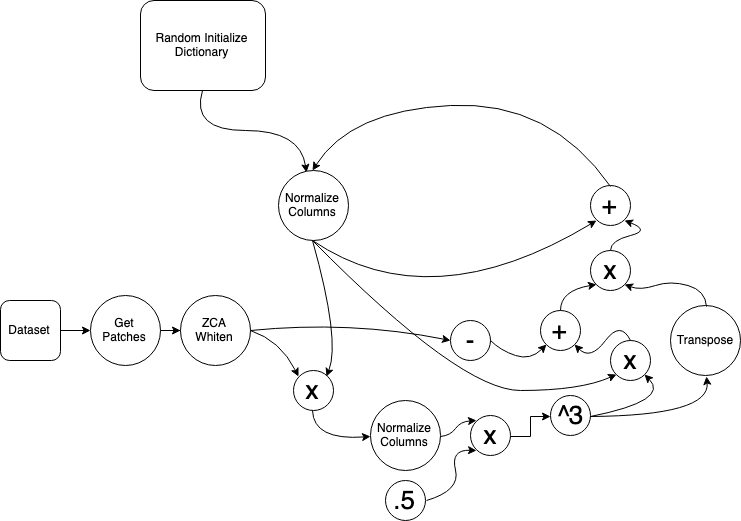
\includegraphics[width=.8\linewidth]{XCubed_diagram}
    \caption{Diagram of XCubed algorithm}
    \label{fig:diagram}
\end{figure}
\begin{figure}
    \centering
    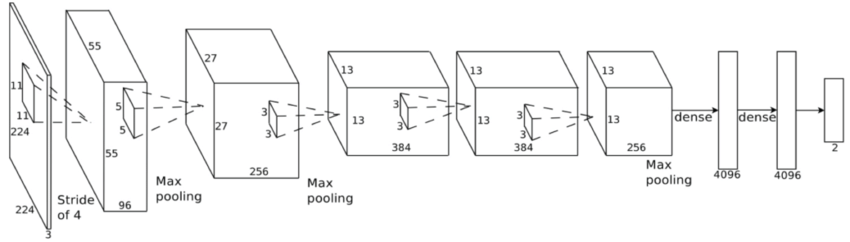
\includegraphics[width=.8\linewidth]{Alexnet_diagram}
    \caption{Diagram of Alexnet CNN}
    \label{fig:alex}
\end{figure}
XCubed is an unsupervised, gradient-free, and loss-free algorithm for generating weights for a convolutional neural network. The algorithm, shown in Figure \ref{fig:diagram}, creates a dictionary of features from patches of your data using a repeated compounding method. We used this algorithm to create convolution features for a neural network. We chose the Alexnet\cite{alexnet} architecture, shown in Figure \ref{fig:alex} for the network as it is a relatively small, simple, and commonly used CNN model\cite{something}. In the first iteration of our network, we ran the XCubed algorithm on the 17 flowers dataset using a patch size of 11x11x3 and set the weights for the first layer of the Alexnet to the output. We then froze that layer and trained the rest of the network with gradient descent. In the second iteration, we went layer by layer running the dataset through the previous layers and running XCubed on the output to generate the weights for that layer. We froze all of the convolutional layers and trained the other layers using gradient descent. In our final iteration, we used the same process but only froze the first three layers.
\section{Results}
\begin{figure}
    \centering
    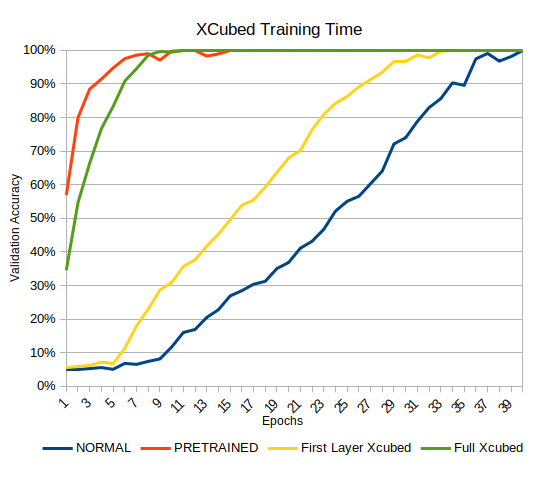
\includegraphics[width=.8\linewidth]{X3GRAPH}
    \caption{Accuracy of various training methods for Alexnet on 17 Flowers}
    \label{fig:netspeedup}
\end{figure}
\begin{figure}
    \centering
    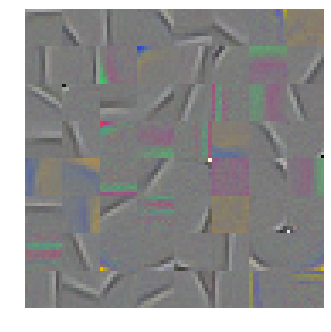
\includegraphics[width=.8\linewidth]{x3filters}
    \caption{Filters produced by XCubed}
    \label{fig:x3weights}
\end{figure}
\begin{figure}
    \centering
    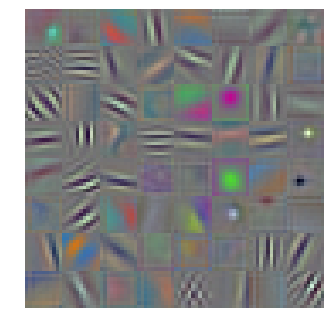
\includegraphics[width=.8\linewidth]{trainedfet}
    \caption{Filters learned by Alexnet's first layer}
    \label{fig:learnedweights}
\end{figure}
The first Alexnet network had its first layer pretrained with XCubed and frozen, and it trained significantly faster than the baseline Alexnet, achieving 99\% accuracy 10 epochs before the regular Alexnet, which was at 90\% accuracy at the time. The second iteration Alexnet did achieve 99\% accuracy, but, although the network started off training faster, it ended up much slower than the baseline due to its inability to train its convolution layers. The Alexnet network where all of the convolutional layers are trained with XCubed and the first three layers were frozen trained much faster than a standard Alexnet or an Alexnet where the first layer is trained with XCubed, with the network reaching 99\% accuracy in just 8 epochs, as shown in Figure \ref{fig:netspeedup}. The training is more comparable to an Alexnet pretrained on imagenet, which starts off with a higher accuracy and reaches 99\% just 1 epoch before at 7 epochs. When run on the Oxford 17 Flowers dataset, the XCubed algorithm produces the first layer filters shown in Figure \ref{fig:x3weights} after 1000 iterations. Alexnet pretrained on imagenet and trained on 17 Flowers produces similar filters, shown in figure \ref{fig:learnedweights}. However, Alexnet had to train fully, while XCubed ran in under 3 seconds on the dataset.

On the ISIC melanoma challenge dataset, our model achieved an accuracy of 73\% in just 45 epochs using a simple Alexnet. The highest accuracy achieved in the 2018 contest without external data was 84\%, and this algorithm would have made 16th place if you do not include entrants who used external data. This model also took less than 3 hours to run on an Intel i5 machine with a Titan X GPU, with the XCubed pretraining only taking 63 minutes and 46 seconds using only the CPU. Interestingly, the first layer features produced by the XCubed algorithm were significantly different from the first layer features for 17 flowers. The features had much more texture features in them such as checker patterns.
\section{Discussion}
%\section{Methods}
%\section{Additional information}
%\section{Data availability}
\section{References}
\bibliographystyle{unsrt}
\bibliography{references}
%\section{Acknowledgements}
%\section{Author information}
%\section{Supplementary information}
%\section{Rights and permissions}
%\section{About this article}

\end{document}